% ===========================================================================
\section{Results}
\label{sec:results}
% ===========================================================================

\subsection{The sector}

The conditional road residual---road transport under the current claimant
assignment---emitted \SI{40.19}{\mega\tonne} \COe{} in FY2023--24 and mixed off-road machinery
\SI{1.73}{\mega\tonne}, together \SI{41.93}{\mega\tonne} on AR5 metrics. The AR6 total is
\SI{41.94}{\mega\tonne}: the two differ by \SI{0.02}{\mega\tonne} because the sector is
\SI{97.4}{\percent} \COtwo{}, whose GWP is unchanged between metrics.

\begin{table}[htbp]
\centering
\footnotesize
\begin{tabular}{@{}lrrr@{}}
\toprule
\textbf{Category} & \textbf{Mt \COe{} (AR5)} & \textbf{AR6} & \textbf{$\pm$\%} \\
\midrule
Road transport (1A3b)     & 40.194 & 40.207 & 11.8 \\
Mixed off-road (1A4c/1A2) &  1.732 &  1.737 & 28.2 \\
\midrule
\textbf{Total}            & \textbf{41.926} & \textbf{41.944} & \textbf{11.4} \\
\bottomrule
\end{tabular}
\caption{Transport-sector emissions, FY2023--24, on the OCAC Road-row controls. Intervals are
parametric and conditional on the claimant boundary; the boundary itself is a structural
axis, priced in Table~\ref{tab:boundary}. The off-road interval is additionally
conditional on the vehicle-kilometre share that carves the class out. The sector band is
narrower than either category's for a directional reason: uncertainty in the road/off-road
\emph{partition} is negatively coupled between the two categories and cancels when they
are recombined, while the control and carbon-factor uncertainties they share are
positively correlated and survive---so the sector inherits only the genuinely shared
terms.}
\label{tab:results}
\end{table}

\subsection{The three fuels}

\begin{table}[htbp]
\centering
\footnotesize
\begin{tabular}{@{}lrl@{}}
\toprule
\textbf{Fuel} & \textbf{Mt \COe{}} & \textbf{Activity basis} \\
\midrule
Petrol                    & 22.542 & OCAC Road row, net of generator petrol \\
Diesel                    & 16.370 & OCAC Road row, net of off-road partition \\
CNG                       &  1.282 & OGRA metered sector gas \\
\bottomrule
\end{tabular}
\caption{On-road emissions by fuel. CNG comes from a different statistic---gas rather
than petroleum---and is the only stream not carved from the Road rows.}
\label{tab:fuels}
\end{table}

CNG is the smallest of the three and the only one not carved from the petroleum controls.
Its \SI{1.28}{\mega\tonne} rests on \SI{62}{} MMCFD of metered gas, converted at a gross
heating value of \SI{1000}{} Btu/scf and then to the net basis IPCC factors are defined on
at \num{0.90}---the gross-to-net convention for natural gas, shared with the captive-power
category and pinned equal to it by test. The heating value is the assumption in the stream,
as it is for captive power, so the alternative is published rather than buried:

\begin{table}[htbp]
\centering
\footnotesize
\begin{tabular}{@{}lr@{}}
\toprule
\textbf{Case} & \textbf{Sector, Mt \COe{}} \\
\midrule
CNG at \SI{1000}{} Btu/scf (reported) & 41.926 \\
CNG at \SI{900}{} Btu/scf     & 41.798 \\
\bottomrule
\end{tabular}
\caption{Pakistani pipeline gas runs \SIrange{900}{1000}{} Btu/scf depending on field and RLNG
share, and nothing read here pins it. The sector moves by \SI{0.13}{\mega\tonne} across the
span---a tenth of the CNG stream.}
\label{tab:cnghhv}
\end{table}

By gas the sector is \SI{40.85}{\mega\tonne} \COtwo{}, \SI{0.67}{\mega\tonne} \NtwoO{} and
\SI{0.40}{\mega\tonne} \CHfour{}, all as \COe{}. That nitrous oxide is nearly twice the methane is
worth noticing: it is a consequence of the off-road factor discussed in
Section~\ref{sec:factors}, and an inventory using the road table throughout would report
roughly a quarter less \NtwoO{} while its \COtwo{} stayed identical.

\subsection{Uncertainty: one reported interval, and its hierarchy}
\label{sec:threeuncertainty}

One interval cannot describe this sector honestly, so the paper reports a hierarchy and
never blends its levels.

\textbf{Reported interval.} $\pm\SI{11.4}{\percent}$ (Approach 1, a
\SI{95}{\percent} relative half-width), \emph{conditional on the current claimant
boundary}. This is the number to quote.

\textbf{Alternative covariance treatments.} The sector's grouped treatment---control and
calorific value shared within each fuel, the fleet term demoted to
distribution-only---gives \SIrange{7.4}{10.1}{\percent} depending on whether the two
petroleum controls, which come from one table of one publication, share one error.

\textbf{Cross-sector shared-factor sensitivity.} The pooled Monte Carlo (Supplementary
Note~S1) reports $\pm\SI{12.9}{\percent}$ under module-shared parameters and
$\pm\SI{12.9}{\percent}$ with the shared fuel-carbon factors correlated across
sectors---the common-random-numbers rebuild made the correlation scenario a no-op for
this sector.

\textbf{The claimant structure, as scenarios.} The boundary itself is a discrete choice
and is never folded into an interval. Table~\ref{tab:boundary} prices it, and reports each
case by category rather than by sector total alone---because for two of these axes the
sector total is the least informative number in the row. The off-road partition cases move
the sector by a rounding error while moving the off-road category by half its own size,
and a reader given only the total would conclude the partition hardly matters.

\begin{table}[htbp]
\centering
\footnotesize
\begin{tabular}{@{}lrrr@{}}
\toprule
\textbf{Case} & \textbf{Road} & \textbf{Off-road} & \textbf{Sector} \\
\midrule
Reference (OCAC Road rows, FY2023--24)   & 40.194 & 1.732 & 41.926 \\
National HSD minus observed bulk rows    & 40.203 & 1.733 & 41.936 \\
Road-share envelope, low (0.864)         & 39.709 & 1.681 & 41.390 \\
Road-share envelope, high (0.908)        & 40.507 & 1.766 & 42.273 \\
Retail non-road at 2.5\% of Road diesel  & 39.785 & 1.732 & 41.517 \\
Retail non-road at 5\%                   & 39.375 & 1.732 & 41.108 \\
Retail non-road at 10\%                  & 38.557 & 1.732 & 40.289 \\
Off-road partition at 5\%                & 40.889 & 0.976 & 41.866 \\
Off-road partition at 15\%               & 39.093 & 2.929 & 42.022 \\
Class intensities at band low            & 40.499 & 1.401 & 41.900 \\
Class intensities at band high           & 40.027 & 1.913 & 41.941 \\
Calendar-2022 controls                   & 47.854 & 2.147 & 50.002 \\
\bottomrule
\end{tabular}
\caption{The boundary and composition axes, structurally
(\texttt{outputs/transport\_uncertainty\_scenarios\_2024.csv}; all Mt \COe{} AR5). The two
defensible constructions agree to \SI{0.04}{\percent} because Road plus domestic bunkers
\emph{is} the national total minus the observed bulk rows. The road-share envelope is a
customer-class boundary sensitivity; the retail non-road rows are the within-channel
sensitivity it cannot provide, and are \emph{transfers} rather than reductions---the
fuel is rebooked to 1A4c\,i, and the national effect is only the trace-gas table
difference, \SI{-0.022}{\mega\tonne} even at \SI{10}{\percent}, because \COtwo{} per
terajoule is identical in both tables. The partition and intensity rows leave the sector
almost unmoved while redistributing between the two categories: that invariance is the
anchoring property, shown rather than claimed. The calendar row is a convention case, not
a candidate: CY2022 straddles the mid-2022 demand collapse.}
\label{tab:boundary}
\end{table}

\begin{table}[htbp]
\centering
\footnotesize
\begin{tabular}{@{}lr@{}}
\toprule
\textbf{Provenance-audit case} & \textbf{Sector, Mt \COe{}} \\
\midrule
Superseded PES control ($\times16/9$)    & 61.524 \\
PES arithmetic corrected, FY2025 vintage & 46.326 \\
\bottomrule
\end{tabular}
\caption{Provenance audit, kept apart from the boundary cases because these are bridges,
not candidates: the first reconstructs the previous edition's published basis exactly, the
second shows what the FY2025-for-2022 vintage mismatch was hiding
(Section~\ref{sec:data}).}
\label{tab:provenance}
\end{table}

\textbf{Composition, bracketed rather than declared.} The class split still has no
independent validation, but it is no longer only a declaration: the declared intensities
that weight it have bands, and moving the whole fleet to either end gives the
class-intensity rows above. Those rows are a \emph{correlated} perturbation, which the
within-fuel normalisation largely absorbs---the two-wheeler share of on-road \COtwo{}
moves by under a percentage point---so reporting them alone would
understate the composition uncertainty. The honest envelope comes from moving classes
against one another: with two- and three-wheelers at one end of their bands and every
heavier class at the other, the two-wheeler share runs several points either
side of the reference---the superseded run's envelope spanned twelve points---and the
rebuilt cases SHIP as scenario rows of the published table
(\texttt{class\_intensity\_low}/\texttt{high} and
\texttt{intensity\_ratio\_light\_low}/\texttt{high} in
\texttt{outputs/transport\_uncertainty\_scenarios\_2024.csv}, beside the
\texttt{class\_split\_declaration} row). Both ends leave every
fuel total exactly where it was. The off-road partition's share is priced by the 5 and
15 percent rows, and the class's agriculture-versus-construction factor mix is
\emph{provably invariant}: IPCC Table 3.3.1's Agriculture and Industry diesel rows are
numerically identical, an executable scenario confirms the zero, and only the road-table
trap (Section~\ref{sec:factors}) moves the answer.

\subsection{Composition, which is what the fleet model determines}

\begin{figure}[htbp]
\centering
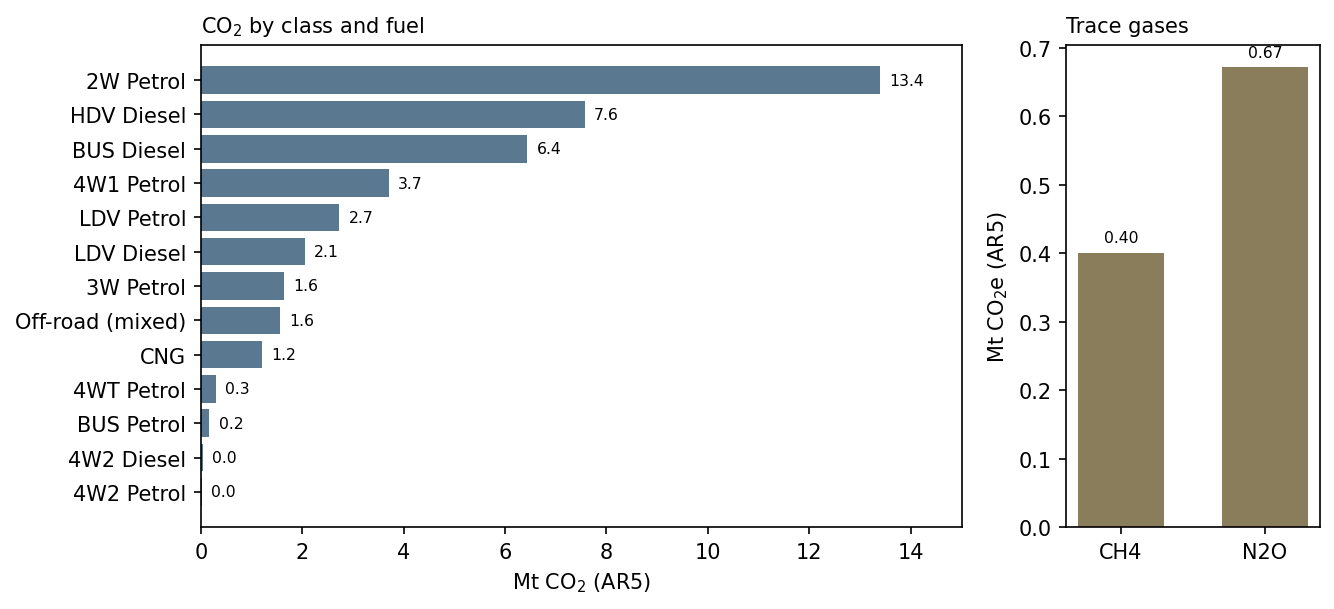
\includegraphics[width=\linewidth]{transport_composition.png}
\caption{\COtwo{} by class and fuel, with the trace gases beside on their own scale.}
\label{fig:streams}
\end{figure}

\begin{table}[htbp]
\centering
\footnotesize
\begin{tabular}{@{}lr@{}}
\toprule
\textbf{Class and fuel} & \textbf{Mt \COtwo{}} \\
\midrule
Two-wheeler petrol          & 13.395 \\
Heavy-duty diesel           &  7.578 \\
Bus diesel                  &  6.441 \\
Four-wheeler (small) petrol &  3.711 \\
Light-duty petrol           &  2.732 \\
Light-duty diesel           &  2.059 \\
Off-road machinery diesel   &  1.569 \\
Three-wheeler petrol        &  1.641 \\
CNG (all classes)           &  1.205 \\
Remaining classes           &  0.522 \\
\bottomrule
\end{tabular}
\caption{\COtwo{} by class, on the energy-weighted allocation. Two-wheelers receive
\SI{34.1}{\percent} of on-road \COtwo{}---still the largest single class, in a fleet
structure that distinguishes Pakistan from most countries whose transport inventories are
used as methodological references, but \emph{less} than heavy goods vehicles and buses
together (\SI{14.02}{\mega\tonne}). A model output, not a measured national finding, and
one this edition changed.}
\label{tab:classes}
\end{table}

\textbf{This table is where correcting the allocation showed up, and the correction
reversed its headline.} The previous edition split each fuel control by vehicle-kilometres
alone, which gives a motorcycle-kilometre the same petrol as a car-kilometre; on that
basis two-wheelers took \SI{42.3}{\percent} of on-road \COtwo{}, \SI{21.9}{\mega\tonne},
and the paper reported them as burning more than heavy goods vehicles and buses combined.
Weighting each class's kilometres by its declared energy intensity moves them to
\SI{34.1}{\percent} and \SI{13.40}{\mega\tonne}, and heavy diesel---trucks and buses at
\SI{14.02}{\mega\tonne}---becomes the larger claim on the sector. The sector total moved by
\SI{0.05}{\mega\tonne} in the process.

That is the third time in this paper's history that reading an input properly has
overturned something it previously reported, after the $\times 16/9$ control arithmetic
and the OCAC tables it described as unobtained while holding them. The pattern is worth
naming rather than quietly fixing: each correction landed in the composition or the
control provenance, never in the anchoring structure, which is the argument for the
structure. It also cuts against the convenient reading of this sector---a
two-wheeler-dominated fleet is a more novel finding than a truck-and-bus-dominated one,
and it was the artefact.

The class table remains the sector's weakest output, and the corrected version is not
better supported than the old one---it is less wrong in a knowable direction. Its three
inputs are registration counts, assumed annual kilometres and declared intensity bands,
none measured in Pakistan. What follows below prices that honestly rather than resting on
the point estimate.

\subsection{The fuel-based series the philosophy makes possible}
\label{sec:series}

The annual road-fuel series covers the same ten fiscal years as the national core, July 2015--June 2025. Fuel controls determine the total; vehicle classes provide a conditional partition. Monthly OCAC editions are held from July 2021. Earlier annual activity is allocated with explicitly weaker support and is not described as observed monthly use. Exhaust timing, evaporation and wear retain their own process evidence labels rather than inheriting one fuel profile universally.

\begin{figure}[htbp]
\centering
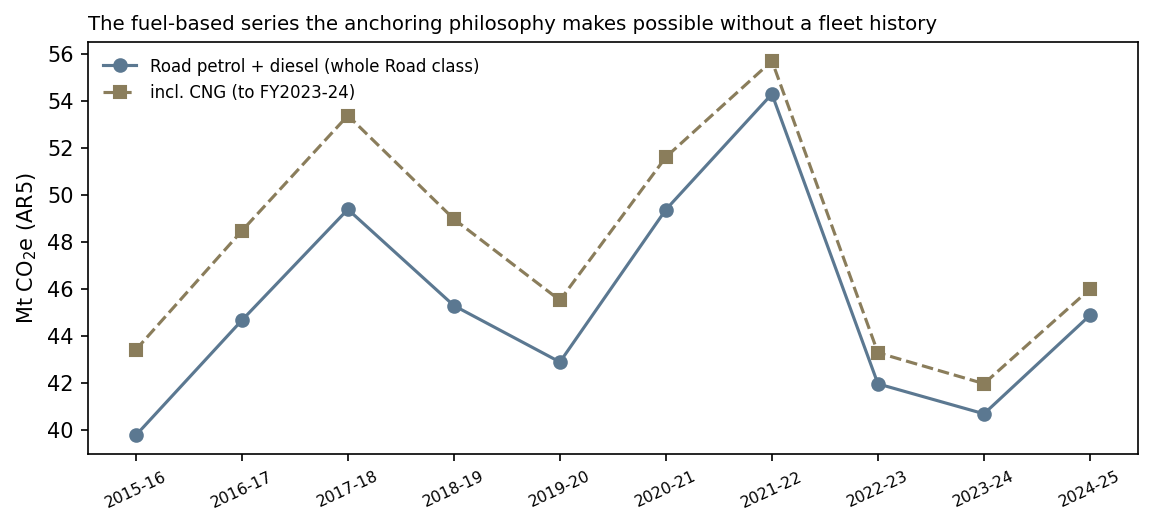
\includegraphics[width=\linewidth]{transport_fuel_series.png}
\caption{Road-class petroleum emissions, FY2015--16 to FY2024--25, with CNG added where
the OGRA series reaches (\texttt{outputs/transport\_fuel\_series.csv}). Whole-Road-class
basis, declared: no generator carve-out back-cast, no off-road partition, no class
composition. The 2022 peak and the post-2022 demand contraction are the feature EDGAR's
own series shows and a fixed-year comparison would have misread.}
\label{fig:series}
\end{figure}

The series is deliberately spartan---whole-Road-class, fuel-based, with a test asserting
its reference-year row equals the inventory's petroleum total modulo exactly the two
declared refinements---because composition over time would require the fleet history the
sector does not have, and inventing it would spend the credibility the fuel basis earns.

\subsection{Provincial allocation, now from fuel sales}

\begin{figure}[htbp]
\centering
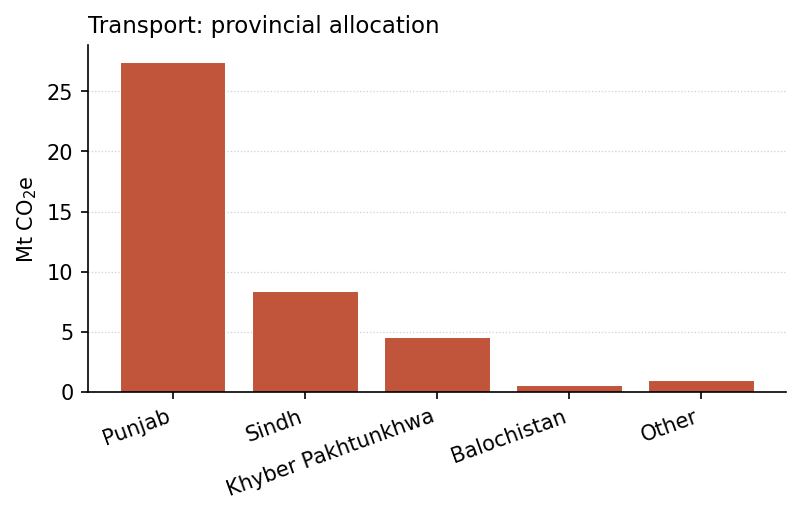
\includegraphics[width=\linewidth]{transport_provincial.png}
\caption{Punjab \SI{27.49}{\mega\tonne}, Sindh \SI{8.36}{\mega\tonne}, Khyber
Pakhtunkhwa \SI{4.52}{\mega\tonne}, Balochistan \SI{0.58}{\mega\tonne}, other
territories \SI{0.98}{\mega\tonne}. The petroleum streams ride provincial fuel sales
from OCAC's monthly area editions, per fuel; CNG and the off-road class ride their own
proxies (Table~\ref{tab:allocwalk}). Fuel sold is still not fuel consumed (freight
crosses provincial boundaries), which is the residual caveat.}
\label{fig:provincial}
\end{figure}

The petroleum streams are allocated on provincial fuel sales---the monthly area pages
of the same OCAC publication the national controls come from, summed and shared per
fuel---replacing the registration proxy whose Sindh result this paper previously
declared indefensible. The shape is the reference year's \emph{own}: twelve FY2023--24
area pages, from OCAC's direct single-month editions
(\texttt{data/activity/transport/ocac\_sectoral\_provincial.csv}).

An earlier edition of this paper borrowed FY2024--25's shape here, on the claim that OCAC
printed complete area pages ``for FY2024--25 and FY2021--22 but not for the reference
period between them''. That was true of the cumulative period-to-date editions the panel
was then built from, which carry a national page only---and false of the publication: the
direct editions of the same months carry full area pages, and the repository held all
thirty-six of them when the sentence was written. The bounding argument offered for the
borrowing was sound---the FY2021--22 bracket bounded it at \num{3.86} percentage
points---and, measured now against the reference year's own pages, the borrowed shape was
in fact off by at most \num{0.45} points on any (province, fuel) share. A sound bound
over a false premise is still not the year's own data. The neighbouring panel years
bracket the own-year shape in
\texttt{outputs/transport\_provincial\_shape\_brackets.csv}, where the largest drift
against either neighbour is \num{3.93} points---the empirical answer, kept published, to
whether borrowing a provincial shape across one year is ever defensible here. Not
every stream rides fuel sales, and Table~\ref{tab:allocwalk} says exactly which does:

\begin{table}[htbp]
\centering
\footnotesize
\begin{tabular}{@{}lll@{}}
\toprule
\textbf{Stream} & \textbf{National control} & \textbf{Provincial proxy} \\
\midrule
Road petrol   & OCAC Road MS+HOBC        & provincial petrol sales \\
Road diesel   & OCAC Road HSD, net of    & provincial HSD sales \\
              & \quad off-road partition &  \\
CNG           & OGRA national metered gas & CNG fleet energy proxy \\
Mixed off-road & HSD partition            & cropland proxy \\
\bottomrule
\end{tabular}
\caption{The allocation crosswalk: which stream rides which provincial proxy. CNG's
geography still rides the fleet model (whose CNG kilometres the two-basis check flags as
overstated), now weighted by the same declared energy intensities as the class split
rather than by distance---three-wheelers are \SI{43}{\percent} of CNG energy against
\SI{74}{\percent} of CNG distance, and the correction moves \SI{4.7}{} points out of
Punjab. The off-road class rides cropland, right for tractors and wrong for the
residual's remainder.}
\label{tab:allocwalk}
\end{table} The change is not cosmetic. Registration location gave Sindh
\SI{6.3}{\percent} of road activity, below Khyber Pakhtunkhwa, for the province
containing Karachi and the port system; fuel sales give it \SI{19.45}{\percent} of road
diesel, and diesel is allocated separately from petrol precisely because freight
geography is not passenger geography.

\begin{figure}[htbp]
\centering
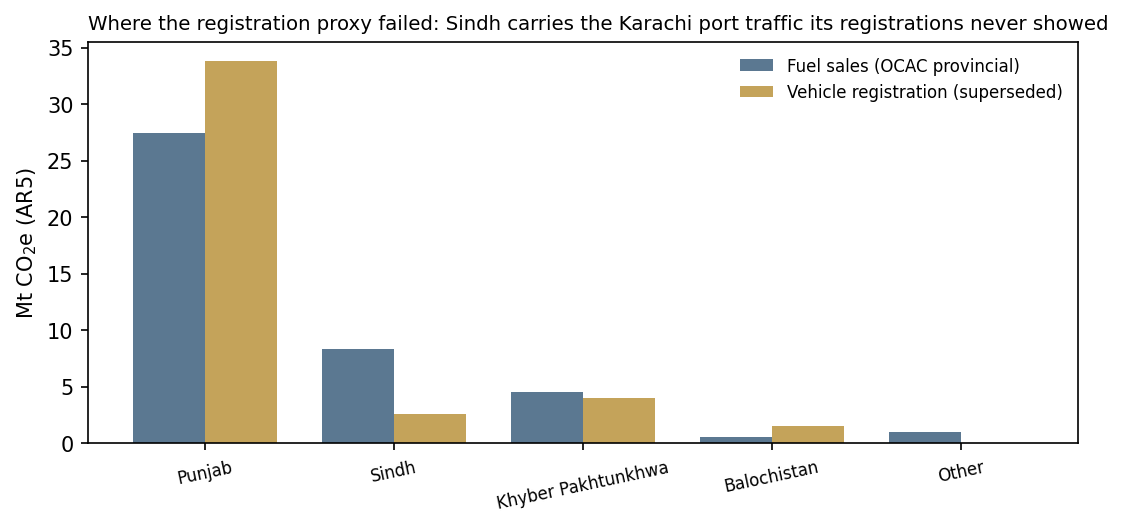
\includegraphics[width=\linewidth]{transport_provincial_proxy_gap.png}
\caption{The failure diagnostic: the superseded registration allocation against the
fuel-sales allocation
(\texttt{outputs/transport\_provincial\_proxy\_comparison\_2024.csv}). Registration
location understated Sindh by roughly a factor of three---vehicles are registered where
it is administratively convenient and fuelled where they work.}
\label{fig:proxygap}
\end{figure}

The remaining caveat is stated rather than hidden: fuel sold in a province is not fuel
consumed there, because freight transits. It is, however, the right error to be left
with---a sales-side blur on a measured quantity, rather than an administrative register
standing in for activity.

\subsection{Contribution to the national inventory}

\begin{table}[htbp]
\centering
\footnotesize
\begin{tabular}{@{}lrr@{}}
\toprule
\textbf{Category} & \textbf{Level (\%)} & \textbf{Variance (\%)} \\
\midrule
Road transport            &  9.04 & 0.90 \\
Mixed off-road (1A4c/1A2) &  0.39 & 0.01 \\
\bottomrule
\end{tabular}
\caption{Shares of the national total and of national Approach-1 variance. At IPCC category level road transportation is the
second-largest category, marginally above public electricity generation; the transport module is
the third largest category of calculation module, behind agriculture and power. It contributes
little to the uncertainty on the national total.}
\label{tab:keycat}
\end{table}

That contrast follows directly from anchoring. Road transport is \SI{9.0}{\percent} of Pakistan's emissions and
\SI{0.9}{\percent} of its inventory variance, a ratio of nearly ten to one in the
direction of "large and parametrically well constrained under the current boundary".

These are COMMON-PERIOD shares, all on FY2023--24. Measured against an FY2021--22 transport year,
the share would be \SI{12.2}{\percent}; on FY2023--24 it is \SI{9.0}{\percent}, and road transport remains
the second-largest category, only marginally above public electricity generation.

That movement is a demand history, not a methods change. Petrol sold to the Road customer
class fell from \SI{9128}{\kilo\tonne} in FY2021--22 to \SI{7209}{\kilo\tonne} in FY2023--24
and diesel from \SI{7887}{} to \SI{5551}{}, so the sector was carrying a figure from the
demand peak that preceded the post-2022 contraction while the sectors it was ranked against
had moved on two years. The previous edition predicted this: it computed the matched-year
share from the fuel series and reported it as \SI{9.43}{\percent} without adopting it. The
realised value is \SI{9.02}{\percent}, and the small remaining difference is the two
refinements the series deliberately omits---the generator carve-out and the off-road
partition.
The reason is structural: the activity datum is a metered, sold, sectorally partitioned
fuel quantity with comparatively narrow bounds, and the emissions are almost entirely
\COtwo{} from a well-characterised factor.

The practical implication is a useful negative result. Refining Pakistan's vehicle fleet model
would improve the class composition---which matters for air quality and for projecting fleet
policy---but would move the national inventory's uncertainty band hardly at all. Fleet
modelling is where transport inventory effort in developing countries usually goes, and on
this evidence it is not where the national total's uncertainty is.
